\section{Results}
\subsection{Localization precision of the microscope}
A set of 100 images of the fluorescent $0.1 \mu$m beads was acquired for each laser wavelength.
An isolated bead was selected and its (two-dimensional) intensity profile was fitted in all images with a (two-dimensional) gaussian curve, using the \verb|curve_fit| \software{Scipy} function. 
The mean and standard variation of the resulting curve provide the $(x,y)$ localisation of the bead and EMPIRICAL PSF
An example of the result of the localization, superimposed on one of the images acquired with the 647 nm laser, is depicted in \autoref{fig:beads_inset_zoom}. 
THUS FOUND EMPIRICAL PSF OF

\begin{figure}[htbp]
    \centering
    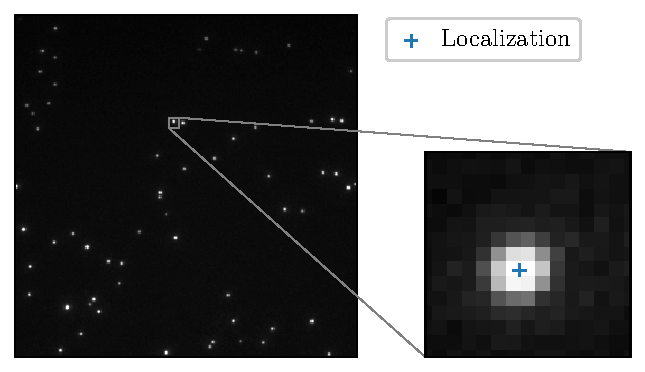
\includegraphics[scale=1]{figures/beads_inset_zoom.pdf}
    \caption{Whole acquisition (647 nm) and zoom on selected fluorescent bead. MUST FIX: la fenetre (les lims) n'est pas la même.}
    \label{fig:beads_inset_zoom}
\end{figure}


\subsection{STORM imaging of micro-tubules}
\begin{figure}[htbp]
    \begin{subfigure}[b]{0.49\textwidth}    % trim left bottom right top
        \centering
        \raisebox{0.5cm}{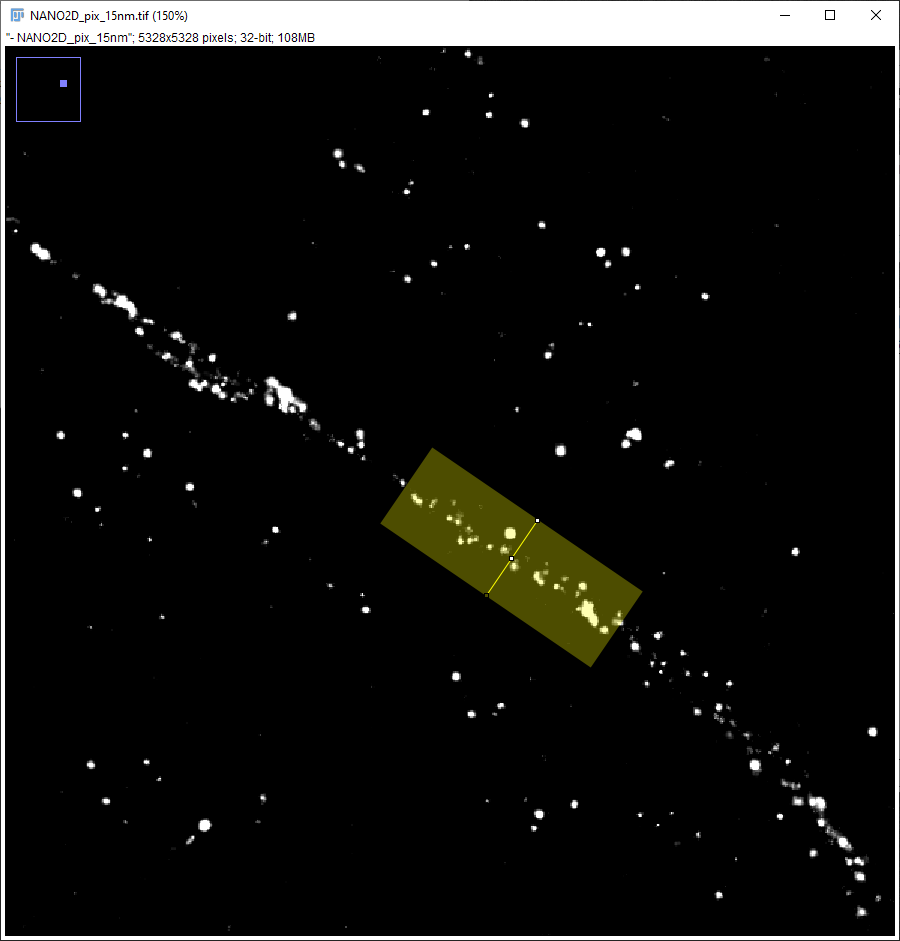
\includegraphics[width=0.9\textwidth, trim={1cm 1.5cm 1cm 5cm}, clip]{figures/microtubules_width_acquisition.PNG}}
        \caption{}
        \label{fig:microtubules_width_acquisition}
    \end{subfigure}
    \begin{subfigure}[b]{0.49\textwidth}
        \centering
        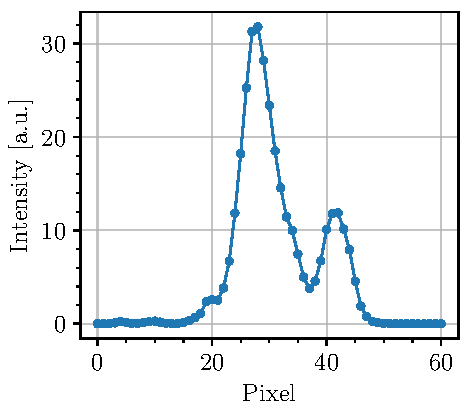
\includegraphics[scale=1]{figures/microtubules_width.pdf}
        \caption{}
        \label{fig:microtubules_width_analysis}
    \end{subfigure}
    \label{fig:microtubules_width}
    \caption{Intensity profile along a microtubule strand: (a) screen capture of the profile acquisition using the \software{Fiji} processing package, (b) the intensity profile averaged over the portion of length considered.}
\end{figure}

\begin{figure}
    \begin{subfigure}{0.32\textwidth}
        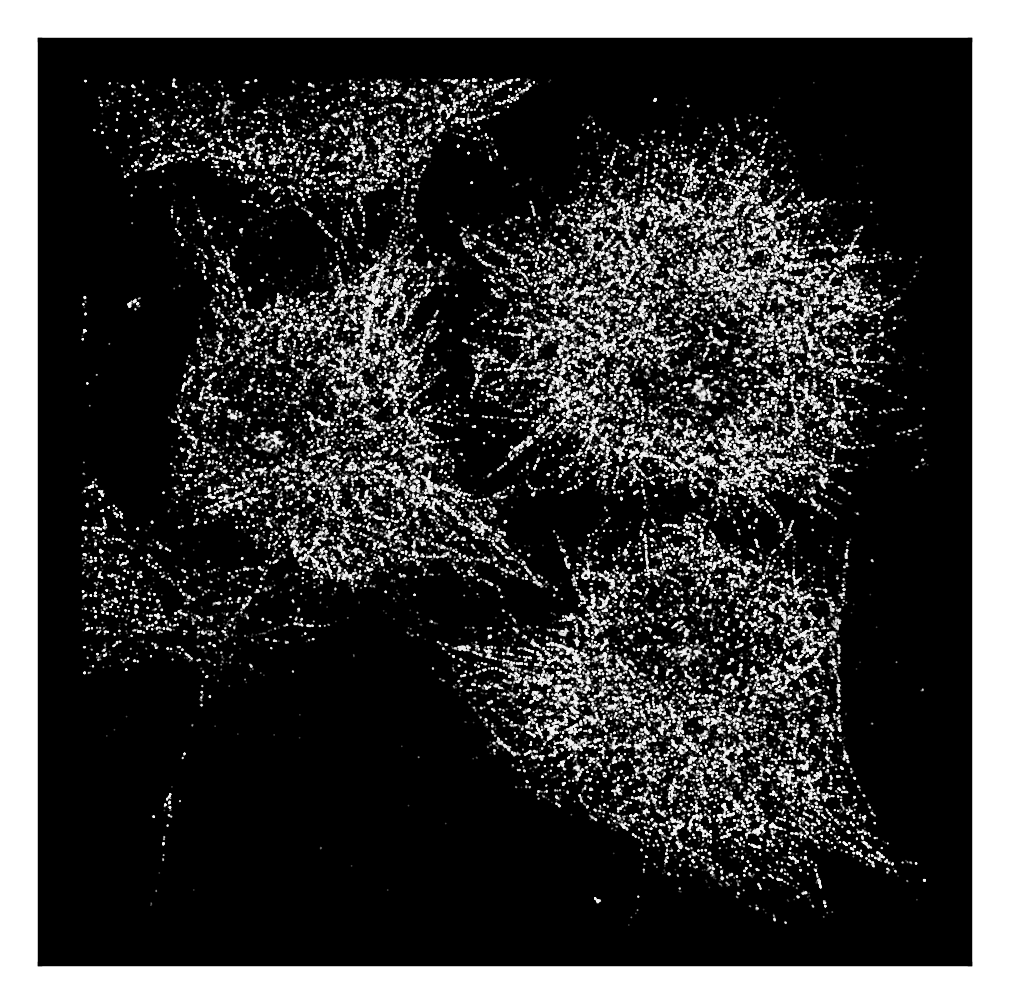
\includegraphics[width=\textwidth]{figures/test_scatter.png}
        \caption{}
    \end{subfigure}
    \begin{subfigure}{0.32\textwidth}
        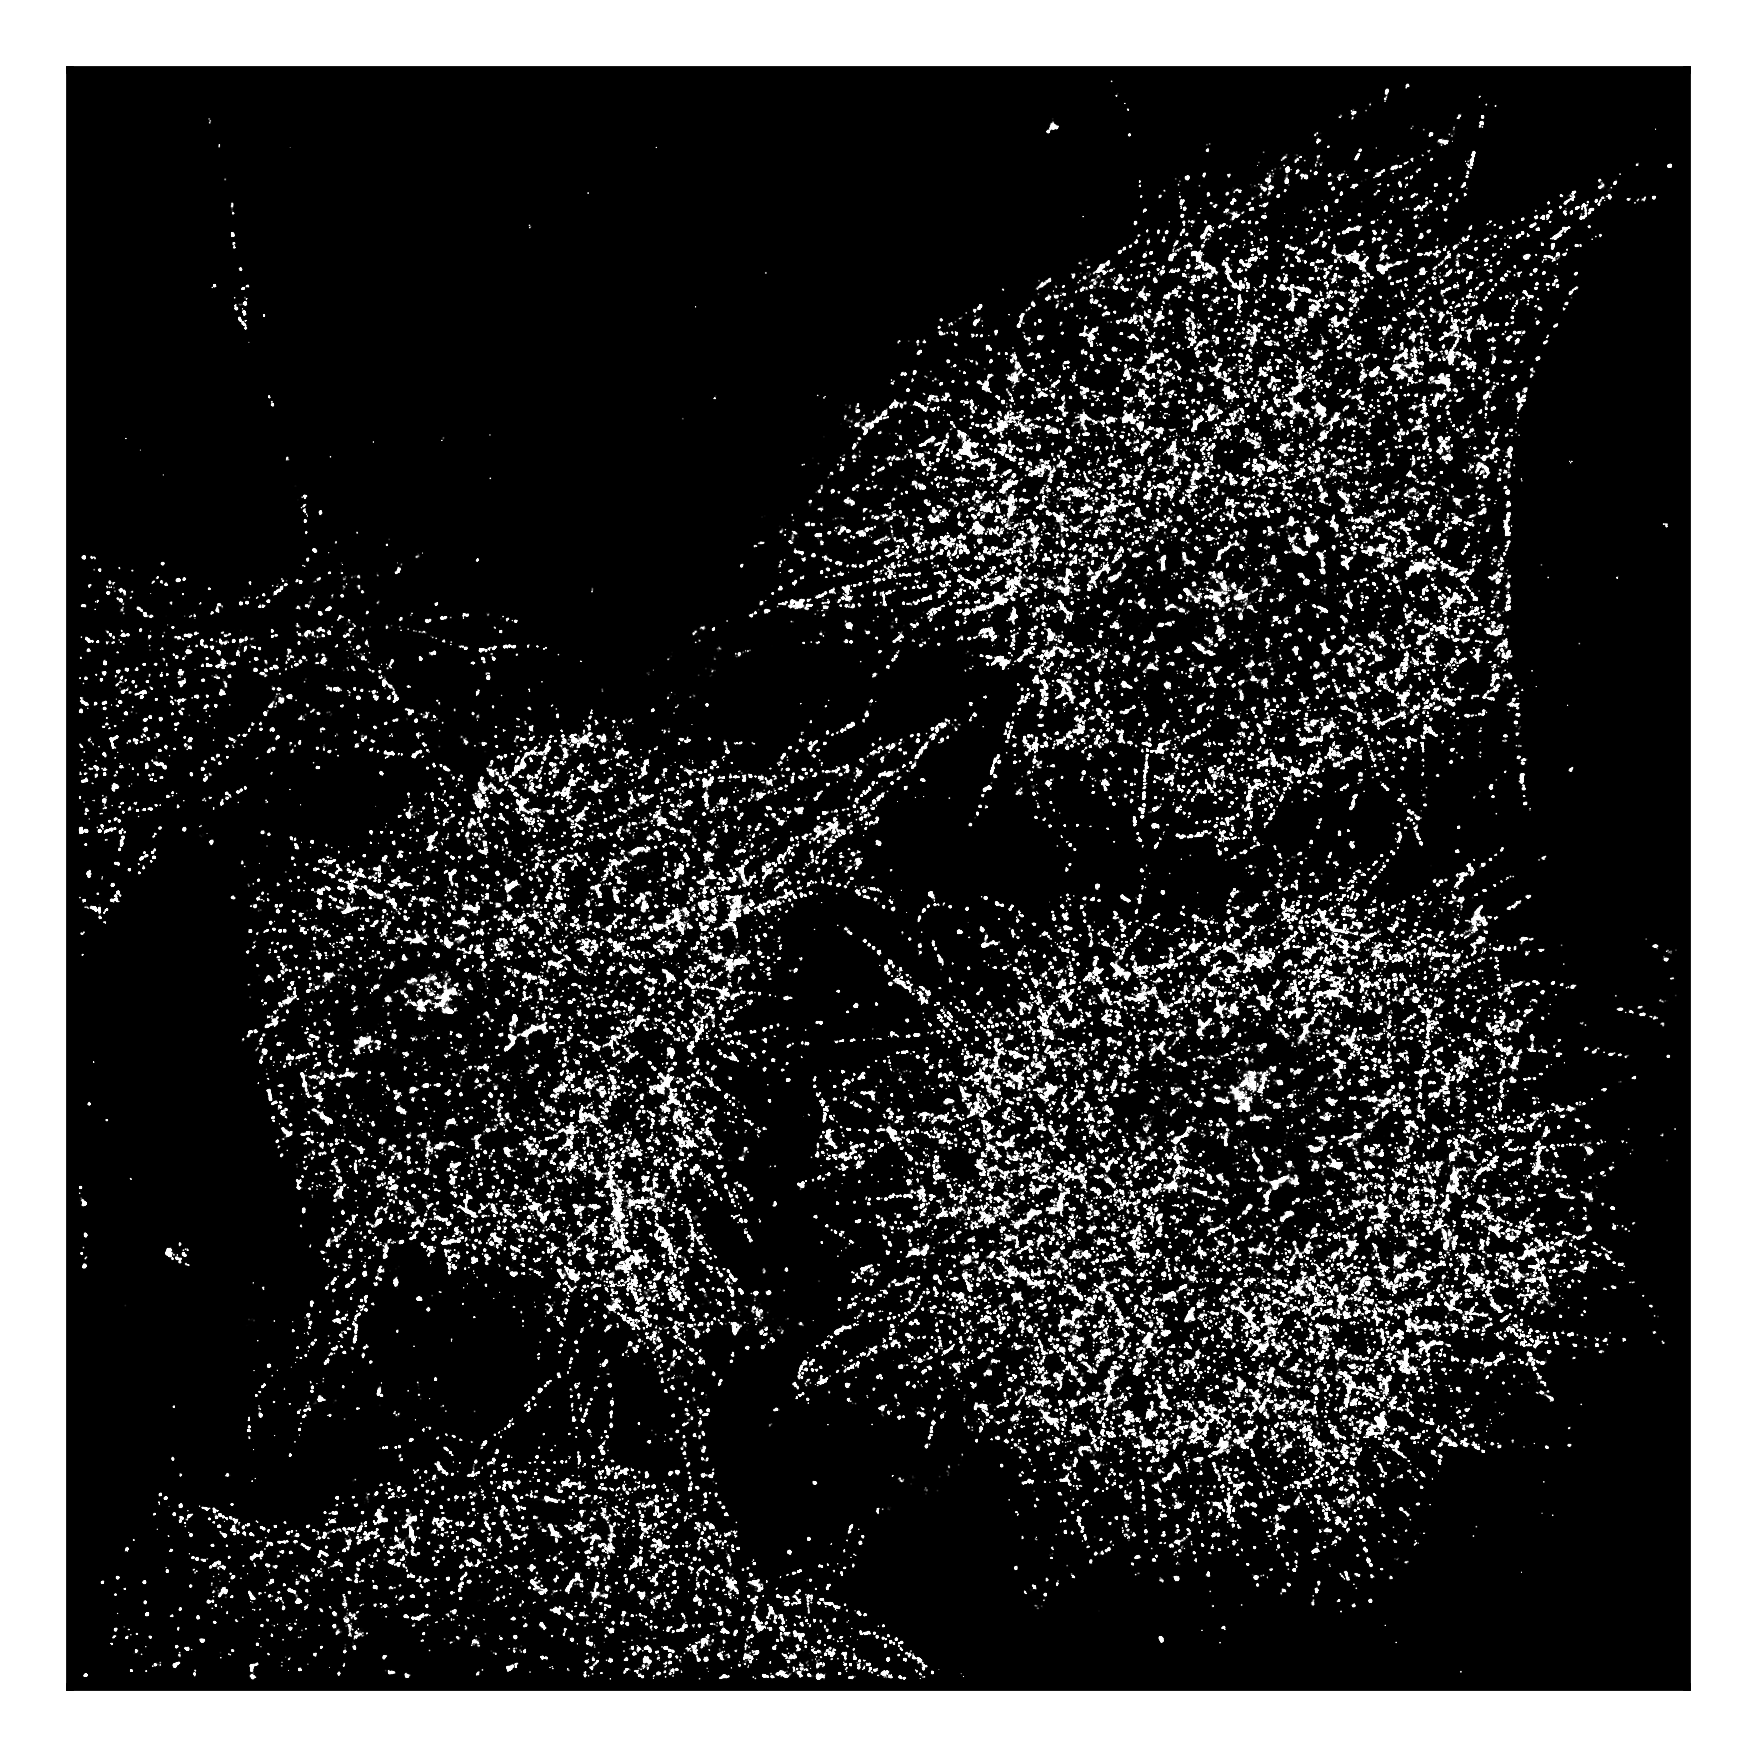
\includegraphics[width=\textwidth]{figures/test_imshow.png}
        \caption{}
    \end{subfigure}
    \begin{subfigure}{0.32\textwidth}
        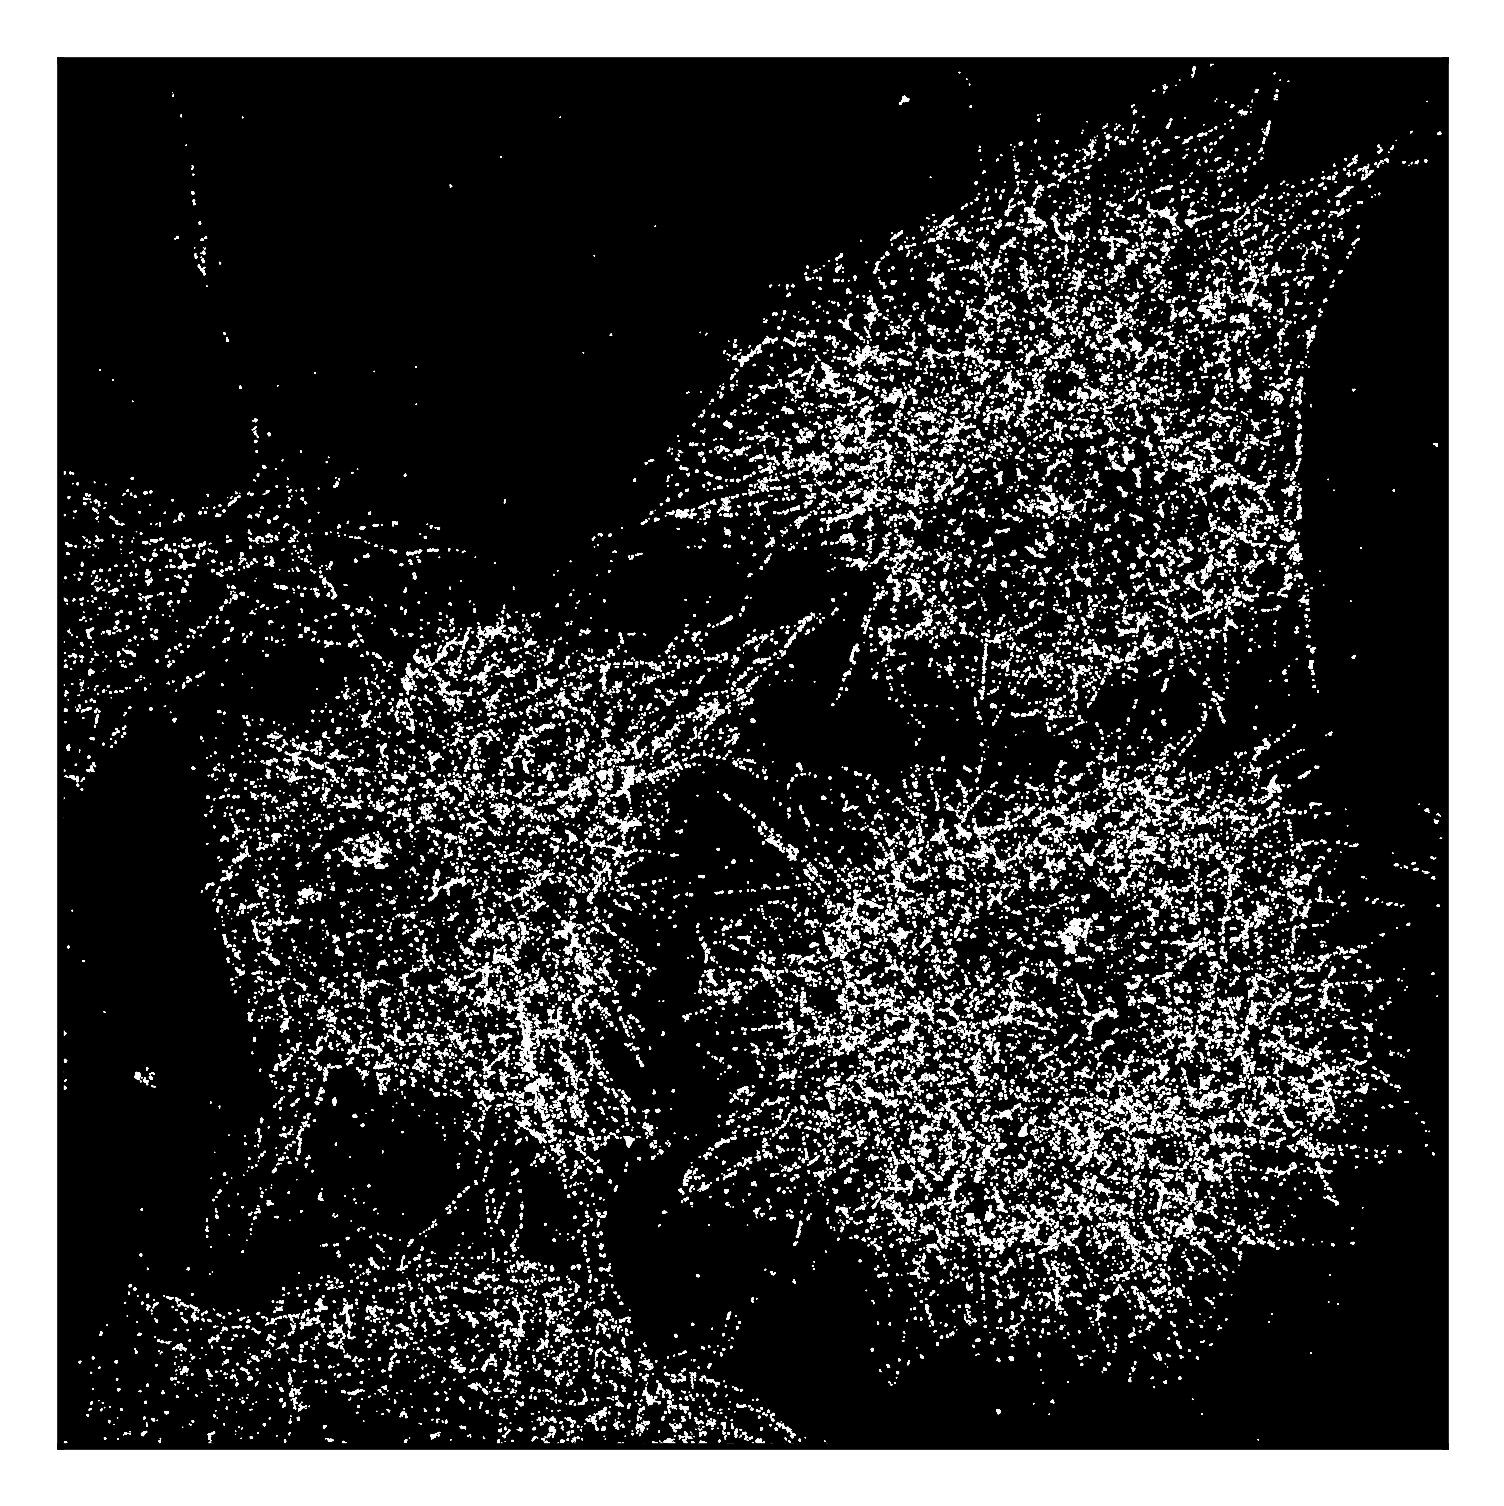
\includegraphics[width=\textwidth]{figures/gaussian_test.png}
        \caption{}
    \end{subfigure}
    \caption{Comparaison des différentes manières de former une image
    (a) scatter, (b) tiff, (c) gaussian magic}
\end{figure}